\documentclass[a4paper, twoside]{report}
\usepackage[utf8]{inputenc}
\usepackage{graphicx}
\usepackage[colorlinks=true, allcolors=blue]{hyperref}
\graphicspath{{images/}}

\usepackage[a4paper,width=150mm,top=25mm,bottom=25mm,bindingoffset=6mm]{geometry}
\usepackage{fancyhdr}
\pagestyle{fancy}
\fancyhf{}
\fancyhead{}
\fancyhead[RO,LE]{Proyecto de Tesis}
\fancyfoot{}
\fancyfoot[LE,RO]{\thepage}
\fancypagestyle{plain}{}

\usepackage{amsmath}
\usepackage[colorinlistoftodos]{todonotes}

\title{Proyecto de Tesis}
\author{Franco Lianza}
\begin{document}

\begin{titlepage}

    \newcommand{\HRule}{\rule{\linewidth}{0.5mm}}

    \center
    
\includegraphics[width=0.4\textwidth]{university.jpg}\\[1cm]

    \textsc{\Large Maestr\'ia en Explotaci\'on de Datos y Gesti\'on del Conocimiento}\\[1.5cm]

    \makeatletter
    \HRule \\[0.6cm]
    {\huge \bfseries \@title}\\[0.4cm]
    \HRule \\[2cm]

    {\Large \@author}\\[3cm]

    {\large Abril 2022}\\[2cm]

    \vfill
\end{titlepage}
\newpage

\subsection*{Tema}
{\it Título del trabajo}

Detecci\'on de los digitos escritos en los telegramas de las elecciones
legislativas en Santa Fe mediante t\'ecnicas de adaptaci\'on de dominio.

\subsection*{Resumen}
{\it Resumen del área sobre la que se realizará el trabajo.}

La rama de {\it Computer Vision} se encarga desarrollar herramientas para
reconocer patrones complejos en im\'agenes en m\'ultiples dominios. Se ha
extendido exponencialmente a lo largo del tiempo, llegando a un punto en el
cual se pueden detectar todo tipo de objetos con una precisi\'on \'optima
\cite{szeliski2010computer}.

Las t\'ecnicas desarrolladas en el \'area precisan de un gran volumen de datos
para su entrenamiento. Esto implica que es de suma importancia de tener
disponibles las {\it labels} (etiquetas) de los datos que se van a utilizar
para entrenar los modelos. El etiquetado de los datos es una tarea costosa,
ineficiente y hasta a veces resulta inviable de realizar \cite{reis2022data}.

A\'un teniendo los {\it labels}, puede ocurrir que el {\it dataset} (conjunto
de datos) donde se va a utilizar el modelo resulte diferente al que se utilizó
para entrenarlo. Por mencionar, un modelo de detecci\'on de rostros entrenado
en una etnia demogr\'afica particular funcionar\'a de manera err\'onea si se lo
aplica a otra. Este fen\'onmeno se conoce como {\it dataset bias} o {\it
		dataset shift} (sesgo en los datos). Dicho de otra manera, un modelo entrenado
en un {\it dataset} puede no generalizar correctamente debido al {\it dataset
		bias}. Algunos autores afirman que el sesgo es un problema que no se puede
evitar al momento de crear un {\it dataset} \cite{khosla2012undoing}.

La detecci\'on de d\'igitos en los telegramas de elecciones en Argentina
podr\'ia llevarse a cabo mediante un modelo entrenado en {\it datasets} de
d\'igitos p\'ublicos como el {\it MNIST} \cite{lecun1998gradient}. Como no
existe una \'unica forma de escribir, el modelo estar\'a sesgado a reconocer
d\'igitos escritos de forma similar a los que se encontraban en el {\it
		dataset} de entrenamiento. No ser\'a capaz de generalizar lo aprendido en un
dominio distinto.

En trabajos anteriores, se aplican distorsiones al conjunto de entrenamiento
para intentar que el modelo pueda generalizar y aplicarse a los telegramas de
elecciones de la Ciudad de Buenos Aires \cite{Lamagna2016}. En el presente
trabajo se utilizar\'an t\'ecnicas referidas al {\it transfer learning},
espec\'ificamente de {\it domain adaptation} para resolver el problema.

El {\it transfer learning} (transferencia de aprendizaje) es un \'area del {\it
		machine learning} que se encarga de almacenar el conocimiento ganado en un
problema y aplicarlo a otro. {\it Domain adaptation} (adaptaci\'on de dominio)
consiste en la habilidad de aplicar un modelo entrenado en uno o mas dominios
de origen ({\it source domain}) en un uno distinto pero relacionado ({\it
		target domain}). La figura \ref{fig:mnist-to-svhn} muestra un ejemplo dos {\it
		datasets} de d\'igitos pero con dominios diferentes. Un modelo entrenado con
	{\it MNIST} no generalizar\'a al conjunto {\it SVHN} por m\'as que ambos sean
d\'igitos.

\begin{figure}[ht]
	\centering
	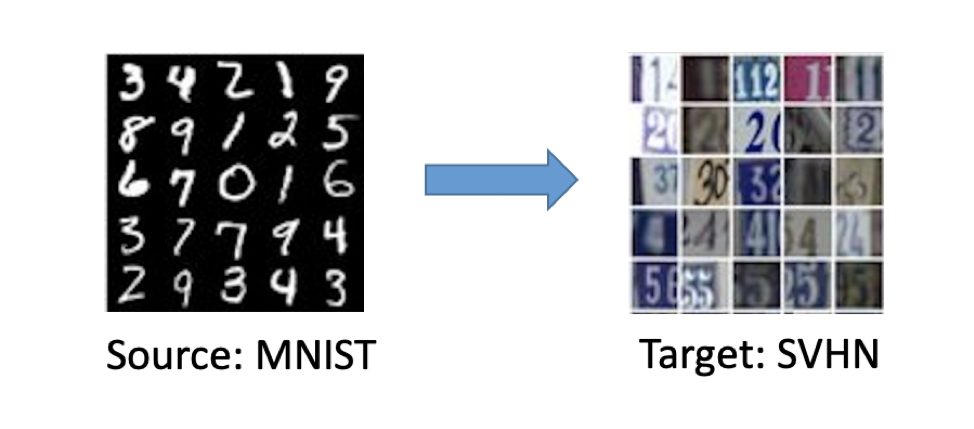
\includegraphics[width=0.6\textwidth]{mnist-to-svhn.png}
	\caption{Ejemplo dominios diferentes: MNIST y SVHN}
	\label{fig:mnist-to-svhn}
\end{figure}

\subsection*{Director o Tutor}
{\it El nombre del director o tutor de la tesis o trabajo, si éste ya
	hubiese aceptado la tarea.}

Dr. Leandro Bugnon

\subsection*{Motivación e importancia del campo}
{\it Explicar la o las motivaciones que llevan a realizar el trabajo planteado
	y su importancia.}

La principal motivaci\'on es obtener un modelo que, basado en un {\it dataset}
similiar, pueda interpretar los d\'igitos de los telegramas de las elecciones
de Santa Fe sin tener de los {\it labels} de los mismos. De esta manera, el
modelo podr\'ia utilizarse en futuras elecciones a fin de automatizar la
digitalizaci\'on de los mismos.

\subsection*{Problemas no resueltos}
{\it Problemas no resueltos detectados en el área y que el trabajo a realizar
	pretende resolver.}

La digitalizaci\'on de los telegramas de las elecciones sigue siendo de forma
manual, lo que genera lentitud y desconfianza en el proceso. Detectar los votos
de manera autom\'atica y reducir la intervenci\'on humana, aumentar\'a la
eficiencia de las elecciones y la confianza en ellas.

\subsection*{Objetivo del trabajo}
{\it Explicar claramente el objetivo del trabajo, especificando su alcance y limitaciones.}

El objetivo del trabajo consiste en detectar los digitos escritos en los
telegramas de las elecciones legislativas de Santa Fe utilizando modelos
entrenados mediante t\'ecnicas de adaptaci\'on de dominio en {\it datasets}
p\'ublicos de d\'igitos.

\subsection*{Requerimientos y desafíos}
{\it Requerimientos y desafíos que plantea el trabajo a realizar.}

El trabajo presenta como principal desaf\'io poder extraer los votos de los
telegramas y analizar distintos modelos utilizando las t\'ecnicas de {\it
		domain adaptation} disponibles. Tambi\'en constar\'a de investigaci\'on
respecto a las {\it Generative Adversarial Networks (GANs)} debido a que varios
algoritmos de {\it domain adaptation} dependen de ellas
\cite{Tzeng_2017,xu2018unsupervised,ganin2016domain}.

\subsection*{Metodología}
{\it Metodología a emplear para el desarrollo del trabajo.}

Los telegramas ser\'an descargados desde la
\href{https://op.elecciones.gob.ar/telegramas/generales2021/}{p\'agina oficial
	del estado argentino}. Luego se extraer\'an los d\'igitos de los votos de cada
telegrama utilizando la librer\'ia {\it OpenCV} \cite{opencv_library}. Una vez
obtenido los digitos, se entrenar\'an distintas redes convolucionales (LeNet
\cite{lecun1998gradient}, ResNet \cite{he2016deep}, etc) utilizando algoritmos
de {\it domain adaptation}. Finalmente, se evaluar\'an los modelos y se
seleccionar\'a/n el/los mejor/es.

\subsection*{Plan de Trabajo}
{\it Especificar las distintas tareas a realizar con los tiempos que se
	estime que deberían insumir.
	Indicar las fechas estimadas de inicio y finalización del trabajo.
}

El trabajo se realizar\'a como consecuencia de la realizaci\'on de las
siguientes etapas:
\begin{itemize}
	\item Investigaci\'on respecto de técnicas de {\it GANs} y {\it domain adaptation}.
	\item Recolecci\'on de telegramas, extracci\'on de d\'igitos y limpieza de los
	      mismos.
	\item Elaboraci\'on de experimentos para el entrenamiento de las redes
	      convolucionales.
	\item Evaluaci\'on y comparaci\'on de los modelos obtenidos.
	\item Redacci\'on final de la tesis.
\end{itemize}

La fecha de inicio del proyecto es Febrero 2022 y como fecha de finalizaci\'on
estimada Septiembre 2022.

\subsection*{Bibliograf\'ia}
{
	%Disable chapter command
	\renewcommand{\chapter}[2]{}
	\bibliographystyle{unsrt}
	\bibliography{refs}
}

\end{document}